\documentclass[letterpaper,10pt,onecolumn]{aspe}

% ===>>> Replace the paper title with yours.

\title{Contact-free, Electrostatically-levitated \\Reticle Handoff in Photolithography Tools}

% ===>>> Replace the author list with yours.
%        Use superscript numbers ($^number$) to identify the correct
%        institution if more than one is being listed below.

\author{Brij M. Bhushan$^1$, David L. Trumper$^1$}%, and Javier J. Author$^2$}

% ===>>> Replace affiliations with yours.  Use leading superscript
%        numbers to identify institutions as they are referred to
%        by the superscript numbers in the list of authors.

\affiliations{$^1$Department of Mechanical Engineering\\
Massachusetts Institute of Technology\\
Cambridge, MA, United States of America}
% $^2$Department or Division\\
% Company or University\\
% City, State or Province, Country}

%   The following packages provide support for figure and math
%   formula and symbol display, leave them in anyway.
%   They are part of LaTeX and should therefore be always available.

%% Font encoding and input file encoding
\usepackage[utf8]{inputenc} %UTF-8 encoded files with the correct header declaration. See https://www.semipol.de/2018/06/12/latex-best-practices.html (donot use with XeLatex, LuaLatex)
\usepackage[T1]{fontenc} % Adds additional characeters not in ACSII (donot use with XeLatex, LuaLatex)

%********** Packages only for abstract ************
% \usepackage{multicol}

\addbibresource{biblio.bib} %Bibliography file

\graphicspath{{./figures/}} % Set the graphics path for use in this chapter

%********************* BEGIN DOCUMENT ***********************
\begin{document}
\maketitle

% \section*{Abstract}

% Context (What you need to know to understand the need)
In semiconductor photolithography, as electronic feature sizes are reducing towards low nanometers, even a few particles on surfaces in the optical path (such as on reticles, lenses, and mirrors) pose critical limits on performance, yield, and machine availability. One of the significant particle generation mechanisms is during object handoff between stages in the manufacturing process. Relative vibration levels between the two stages cause impact forces and relative sliding between surfaces leading to wear and particle generation. Unlike in air, non-contact solutions like Bernoulli grippers do not work in vacuum.
% In extreme ultraviolet (EUV) photolithography, reticle exchanges have been shown to contribute to the loss of productivity and reticle wear. Reticle exchanges have also been linked to an increased defect rate on the reticles. 
Currently, in extreme ultra-violet (EUV) lithography machines, an electrostatic chuck with a six-degree-of-freedom (6-DOF) short-stroke stage aligns and moves relatively slowly until it contacts the reticle carried on a reticle exchange device (RED) arm. The challenges of the current mechanical handoff are: 1)~poorly-defined control of the contact attitude and mechanics; 2)~a trade-off between contact forces and the handoff time, as the impact forces depend on the relative velocity at the time of contact;
% with vibrations setting the lower bound of the contact forces;
% Furthermore, the relative vibration levels between the RED arm and the electrostatic chuck place a lower bound on the velocities and impact forces. 
3)~The reticle corners make the first contact with the chuck due to a slight bow in the reticle from its self-weight of the order of \SI{1}{\micro m}.
% At that time, the reticle center does not make contact because of the bow. 
Then, when the chuck turns on to a high voltage, the reticle bow flattens and the corners and edges scrape against the chuck surface until the reticle makes uniform contact. All the above challenges increase wear and particle generation.
% The relative motion at the edges and corners leads to potential particle generation and accelerated wear of the reticle and chuck.

% Need (A way to motivate the audience (what you have != what you want))
As the industry moves towards double patterning with EUV, faster reticle exchanges with lower wear and particle generation become even more critical. Our solution is to convert the transfer problem from a three-body contact (handoff stage, object, and pickup stage) to a phased two-body contact during transfer by electrostatically levitating the object during handoff.
% Task (What I decided or was asked to do in order to address the need)
We explore various sensing and actuation patterns, develop control strategies, and evaluate methods to avoid electrostatic discharge during stable levitation and reticle handoff between the chuck and the RED arm. We demonstrate the proof of concept in air by levitating a \num{152} by \SI{152}{mm}, \SI{400}{\micro\meter} thick aluminum sheet over \SI{200}{\micro\meter} air-gap.
% Object (What the document does/contains (and what you should do with it))
This paper describes the design of the testbed and presents the experimental results.
%%% Reader asks: Do I care? Have you answered this question above?
% Findings (What I found as a result of carrying out the task)
The setup actively controls the position of the floater in 3-DOF (air-gap in the vertical direction, \(\mathrm{Z}\), and rotations, \(\mathrm{\theta_x}\) and \(\mathrm{\theta_y}\)) and the flexible \(\mathrm{Bow}\) shape of the floater. The 3-DOF in horizontal directions (\(\mathrm{X}\), \(\mathrm{Y}\), and \(\mathrm{\theta_z}\)) are passively controlled. The position of the floater is controlled to within \SI{200}{nm-pp} in the \(\mathrm{Z}\)-direction and \SI{0.2}{mdeg-pp} in \(\mathrm{\theta_x}\) and \(\mathrm{\theta_y}\) directions with about \SI{100}{Hz} maximum crossover. The horizontal positions are repeatable to better than \SI{\pm 0.5}{mm} in \(\mathrm{X}\) and \(\mathrm{Y}\), and \SI{\pm 0.2}{deg} in the \(\theta_z\) direction.
We successfully demonstrate pickup, clamp and unclamp, place-down sequences by moving the floater from the resting pins about \SI{200}{\micro\meter} away to the electrodes and back.

% Conclusion (What the findings mean to you (possibly what you should do) | Interpretation/Recommendation)
In our setup, we demonstrate the concept of non-contact levitation and transfer of the reticle establishing a small upward bow shape such that the first contact is at the reticle center and then flattens outward. This addresses the challenges described above, as the system: 1)~is relatively insensitive to starting positions, orientations, and vibrations;
% Once the reticle is in suspension, the reticle vibrations are mainly from the sensing noise attached to the metrology frame, ideally the same frame as the electrostatic chuck; 
2)~has lower impact forces due to lower moving mass for the same velocity of contact, resolving the contradiction between the time required for reticle exchange and wear and particle generation;
3)~makes first mechanical contact at the center of the reticle minimizing shear motion between the reticle and chuck.
% Perspectives (What I/you/they will do in the future)
The concept and design methodology for contact-free object handoff described in this paper can be extended, using various actuation methods such as electrostatics, electromagnetics, and pneumatics, to other situations where wear and particle generation from object handoff are critical.

%%% Reader asks: Do I need more? Is the work relevant to read the rest of the paper?

\vfill
{\small Acknowledgement: This work is supported by \href{https://www.asml.com/en}{ASML US LLC} under grant number xxx.}

\newpage
\twocolumn[] %Start next page with two column for multiple figures

\begin{figure}
    \centering
    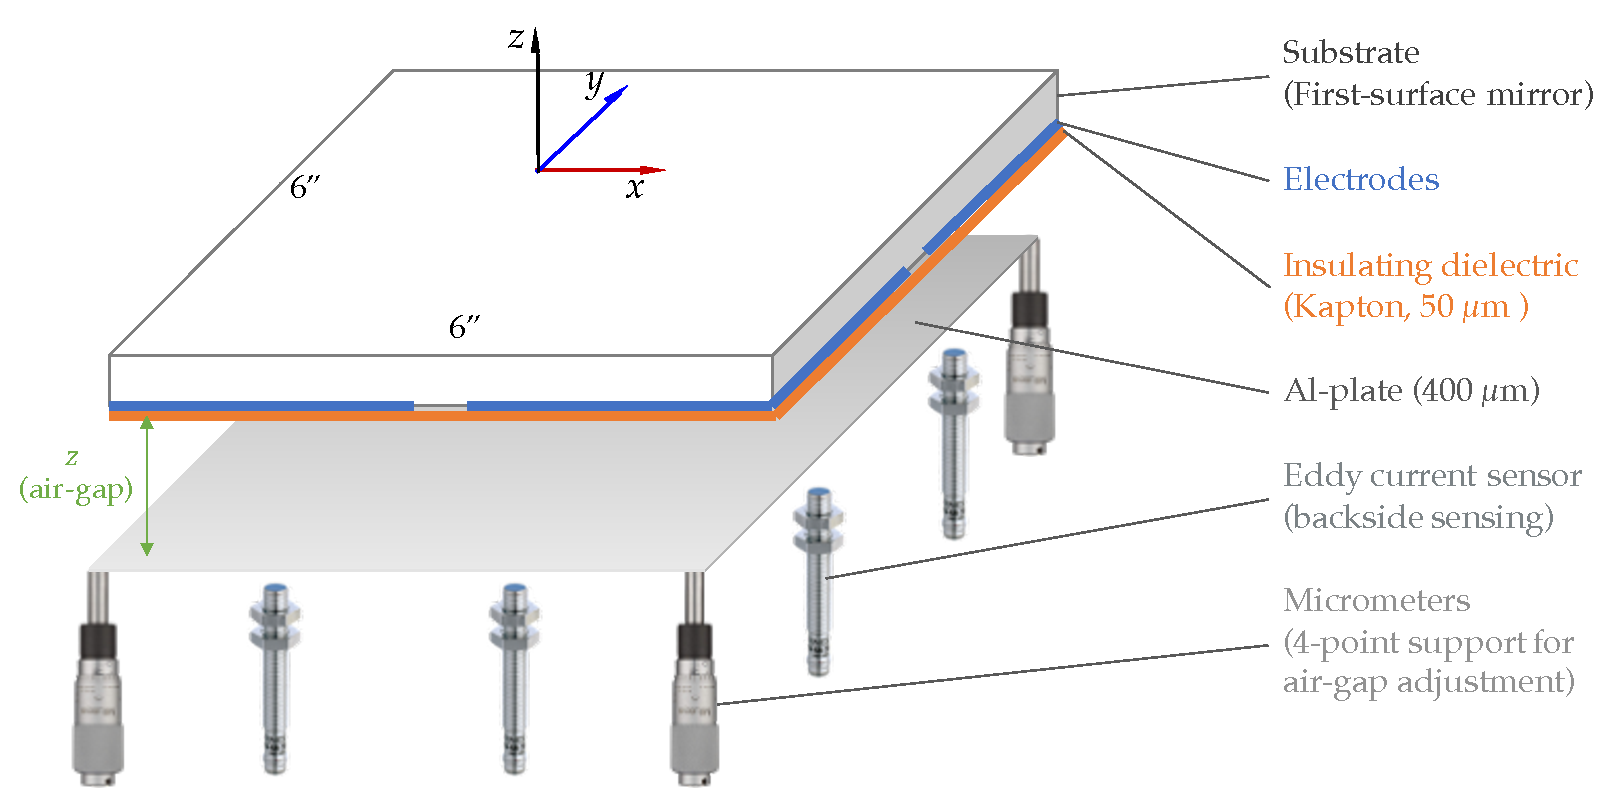
\includegraphics[width=\linewidth]{ConceptSchematic.pdf}
    \caption[]{Conceptual Schematic of the 6-DOF setup.}\label{fig:ConceptSchematic}
\end{figure}

\begin{figure}
    \centering
    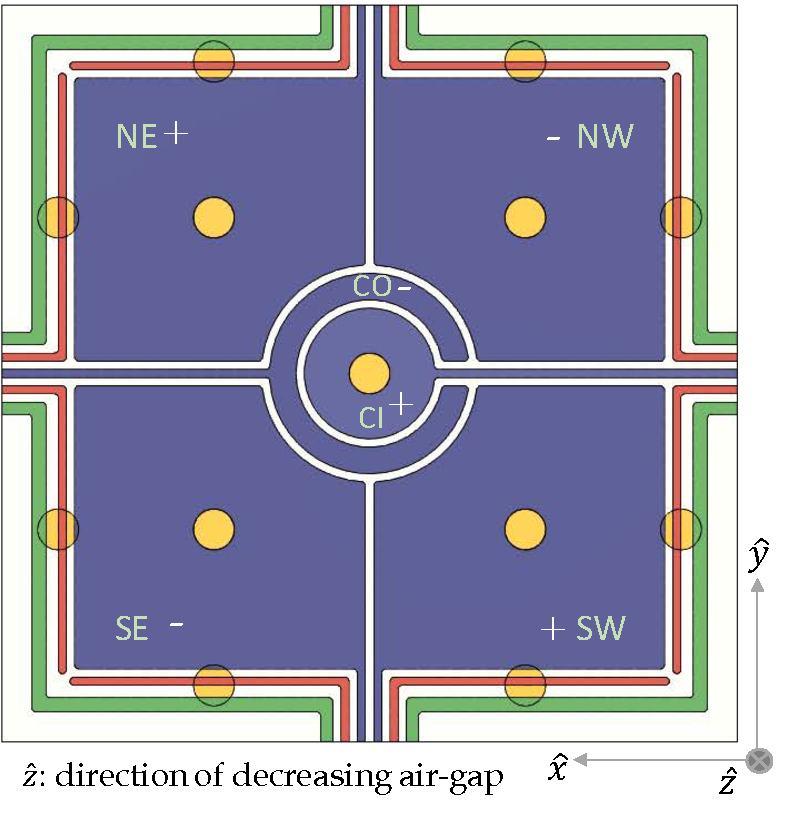
\includegraphics[width=0.8\linewidth]{Electrode_eddy_pattern.pdf}
    \caption[]{Electrode layout and eddy current sensor pattern. The main electrodes are in blue, the ring electrodes in red, and the ground electrodes are in green. Yellow circles show the eddy current sensor positions. The polarity of the main electrodes are indicated by \(+\) and \(-\) signs. The connections to the high voltage amplifiers are through the electrode leads to the edge of each side of the first-surface mirror.}\label{fig:electrode_pattern}
\end{figure}

\begin{figure}[!b]
    \centering
    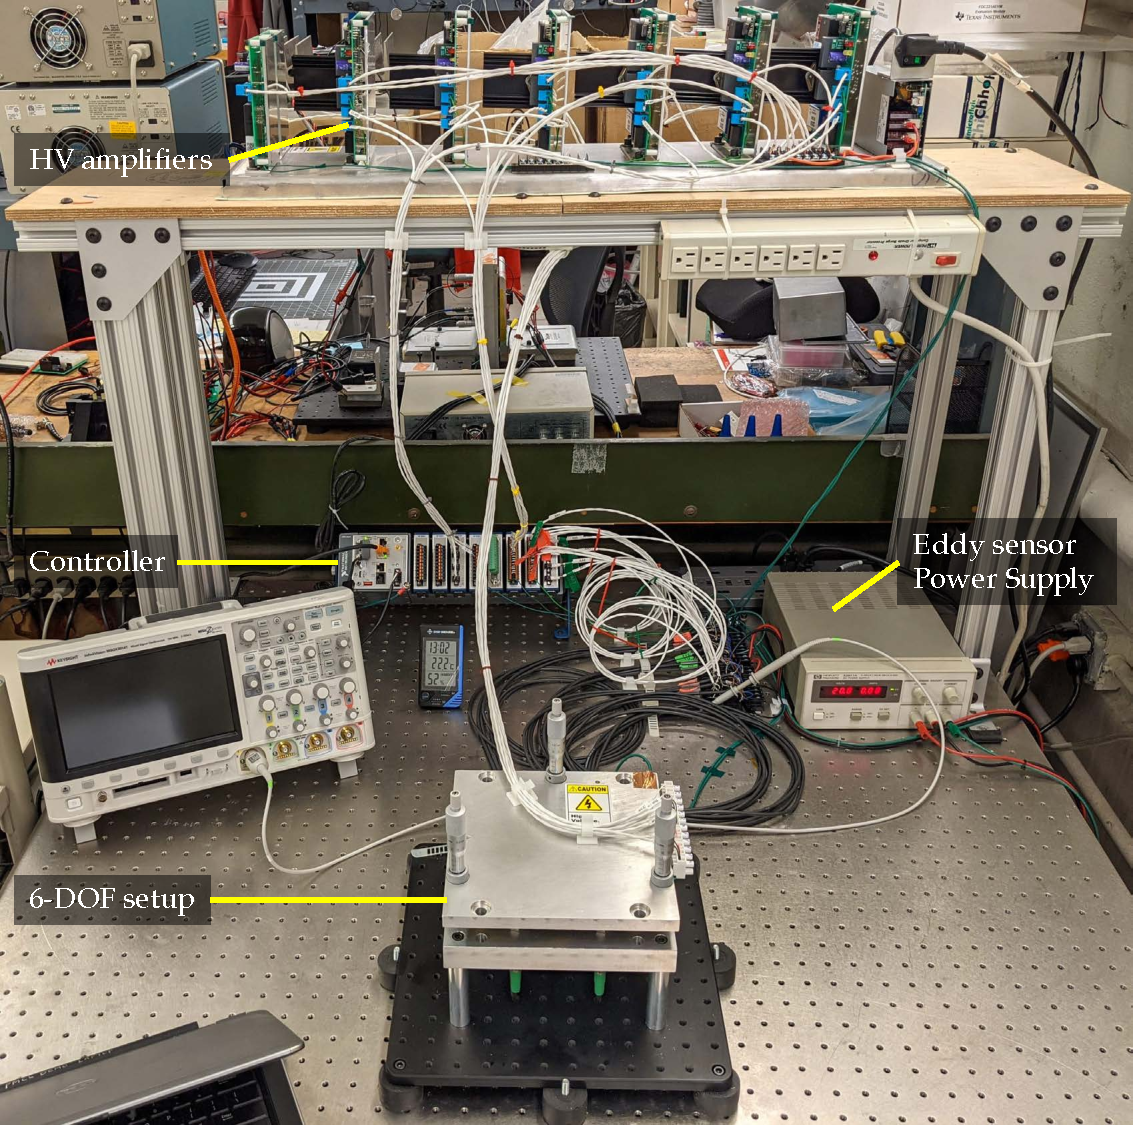
\includegraphics[width=0.95\linewidth]{6DOF_Levitation_Setup_labels_v3.pdf}
    \caption[]{6-DOF experimental testbed showing various parts of the system. }\label{fig:6-DOF_setup_full}
\end{figure}

\newpage

\begin{figure}
    \centering
    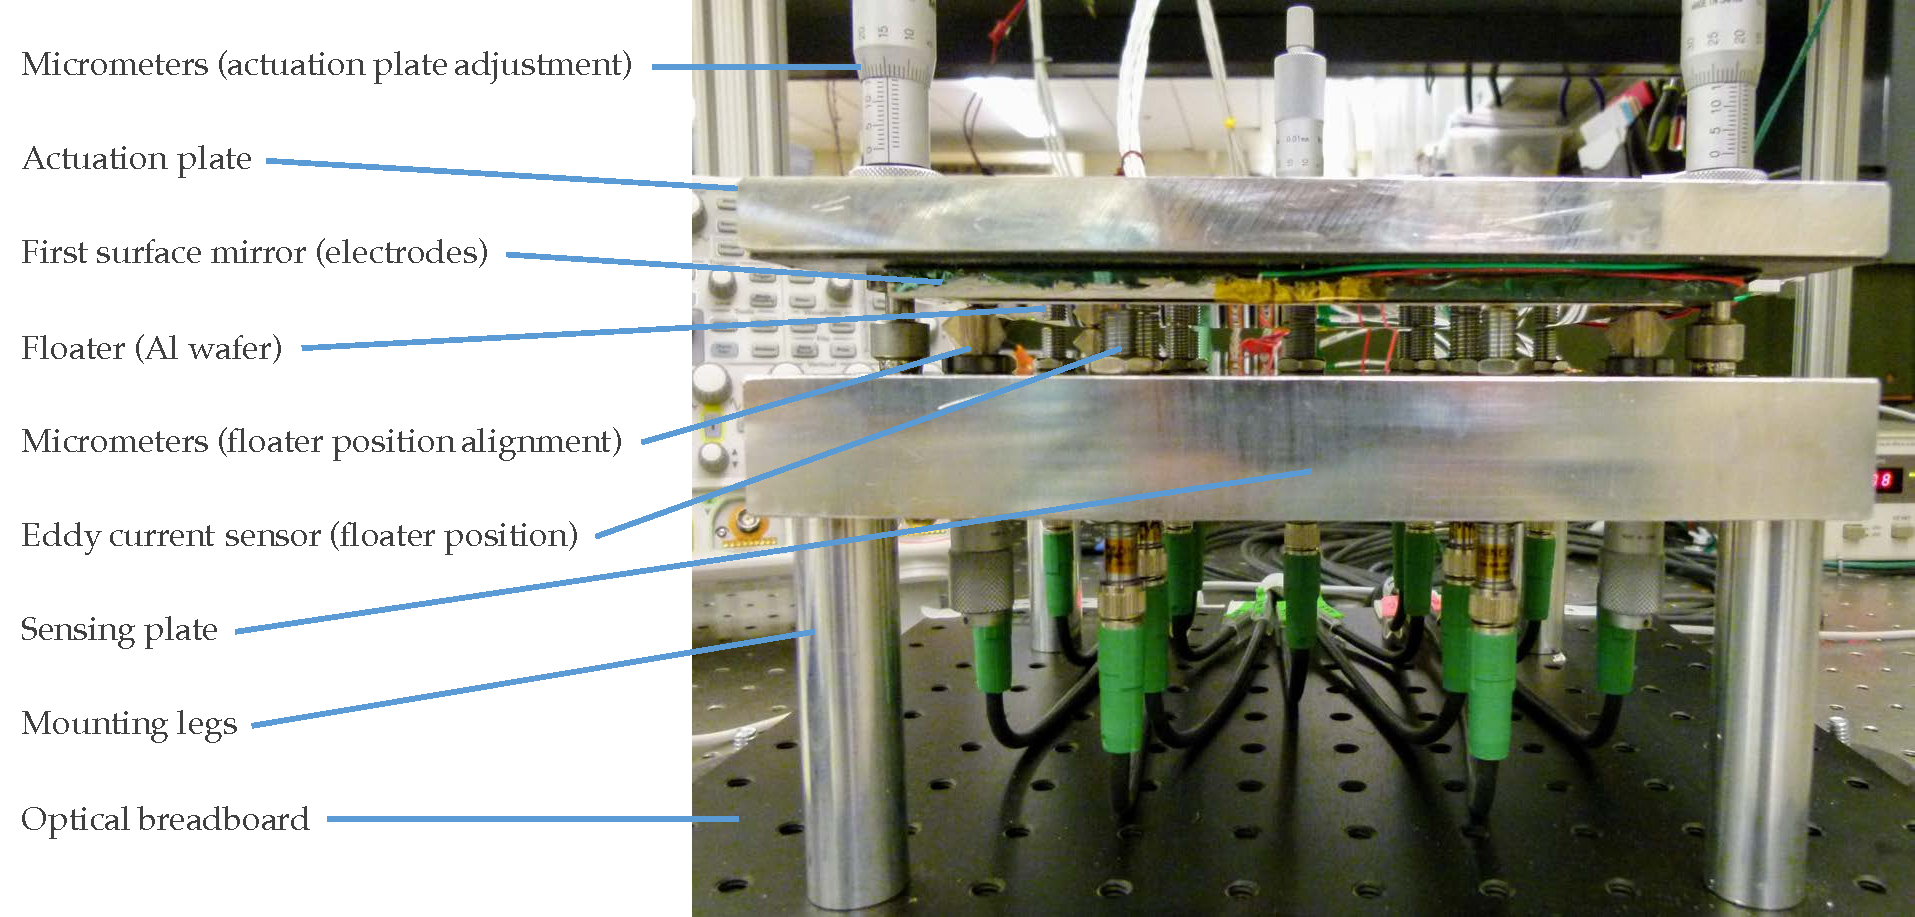
\includegraphics[width=1\linewidth]{6-DOF_setup_labels_v2.pdf}
    \caption[]{6-DOF setup front-view of the hardware.}\label{fig:6-DOF_setup}
\end{figure}

\begin{figure}
    \centering
    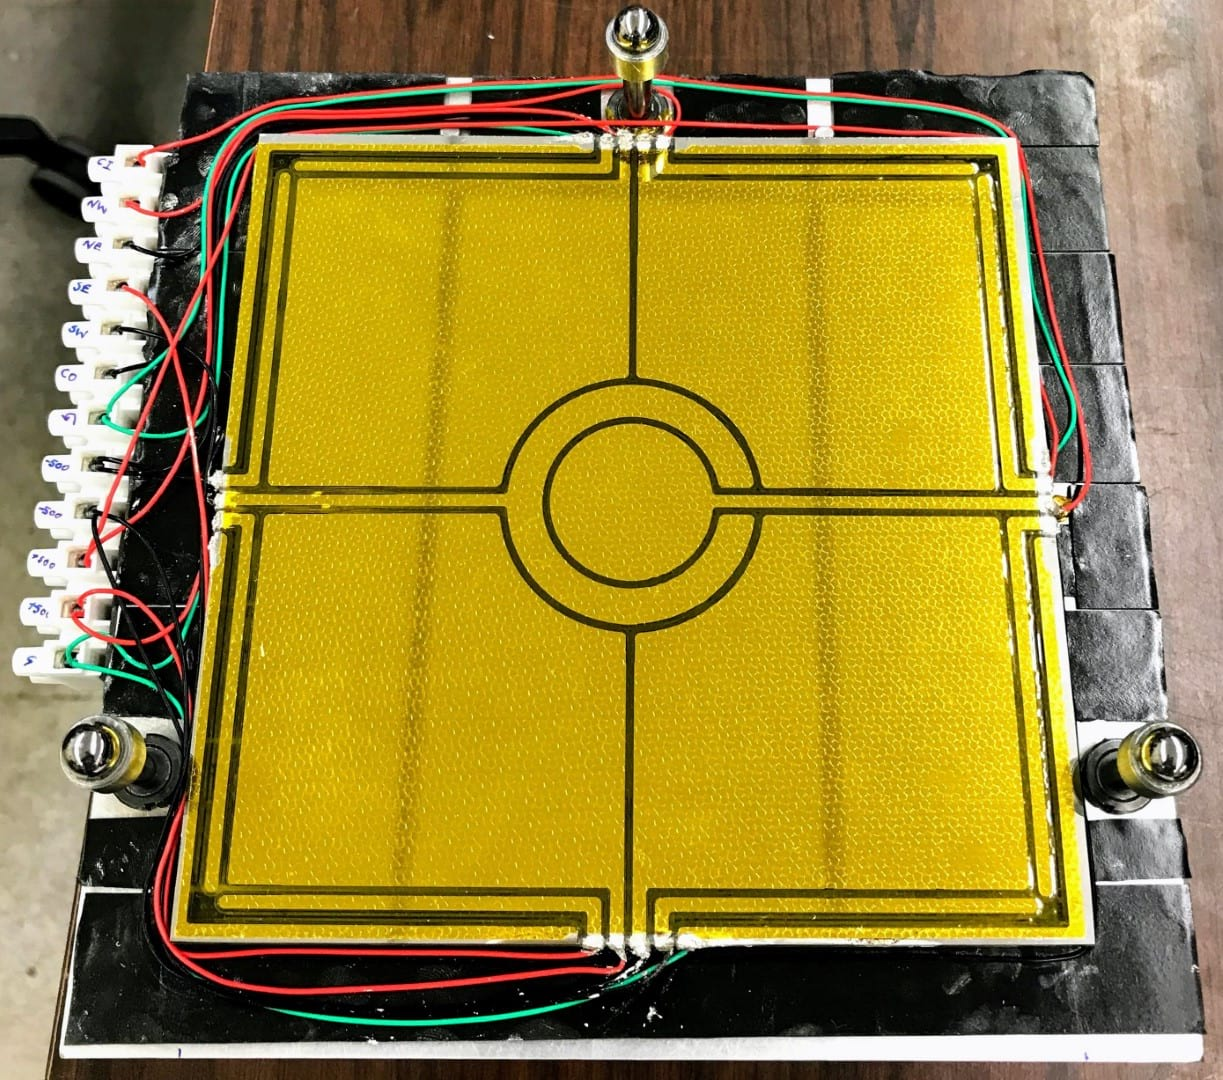
\includegraphics[width=0.65\linewidth]{electrodes_fabricated.jpg}
    \caption[]{Fabricated electrode assembly.}\label{fig:electrodes_fabricated}
\end{figure}

\begin{figure}
    \centering
    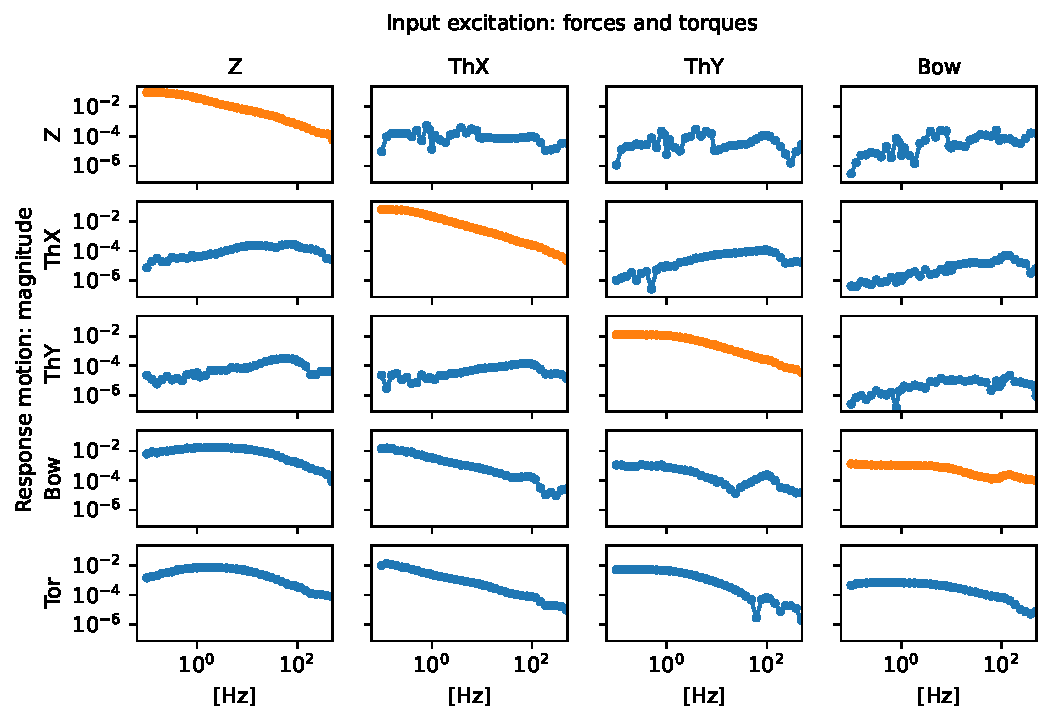
\includegraphics[width=1\linewidth]{Plant_BodeMagMatrix.pdf}
    \caption[]{Plant Bode plot matrix for excitation and response in all the modes. Only magnitudes are shown for clarity.}\label{fig:plant_BodeMatrix}
\end{figure}

% \begin{figure}[!b]
%     \centering
%     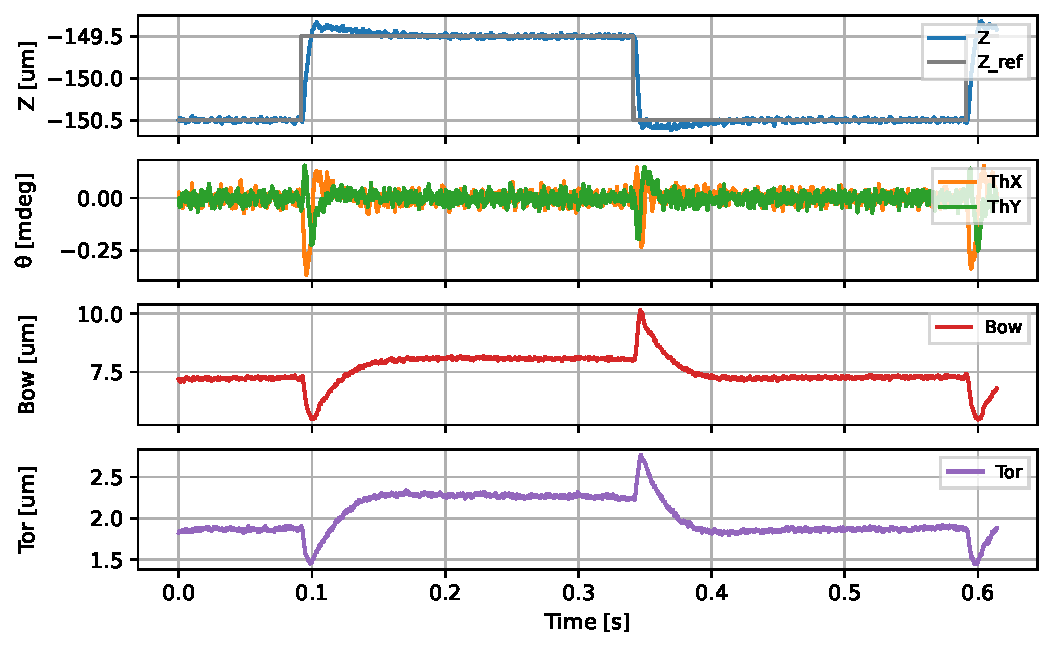
\includegraphics[width=0.9\linewidth]{150_Zsquare.pdf}
%     \caption[]{Z-direction step response at \SI{150}{\micro m} air gap for a \SI{1}{\micro m} step.}\label{fig:step_response}
% \end{figure}

\begin{figure}[!b]
    \centering
    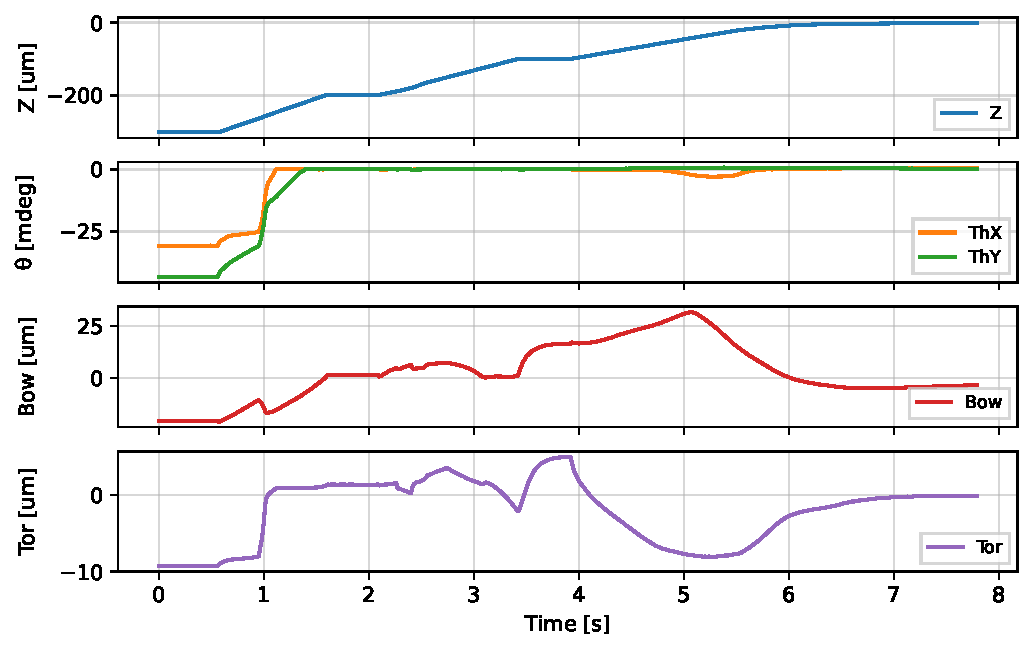
\includegraphics[width=0.9\linewidth]{floater_pickup_clamp.pdf}
    \caption[]{Floater pickup and clamp demonstration. Starting position at \(\mathrm{Z}\) of \SI{-300}{\micro \metre}, with \SI{-30}{\milli deg} and \SI{-45}{\milli deg} of tilt in \(\mathrm{\theta_x}\) and \(\mathrm{\theta_y}\). \(\mathrm{Bow}\) of \SI{40}{\micro \metre} with center making first contact. }\label{fig:floater_pickup_clamp}
\end{figure}

\newpage

%%%% Template LaTeX code below for use with writing the extended abstract manuscript

% \section*{Background theory}
% Oversampling refers to the process of sampling a signal at a significantly higher rate than the Nyquist frequency \cite{WikiOversampling}. In feedback control applications, oversampling refers to sampling the sensor signal much faster than the control loop rate. Oversampling is capable of improving the resolution and signal-to-noise ratio (SNR) and hence, the dynamic range (DR) within the control loop bandwidth. A high SNR and high DR are important requirements of sensing for mechatronic systems with closed-loop feedback. \cite{Oppenheim2013}. See Fig.~\ref{fig:example_fig} for an example figure.

% \begin{figure*}
%     \centering
%     \hspace*{\fill}%
%     \begin{subfigure}[b]{0.5\textwidth}
%         \centering
%         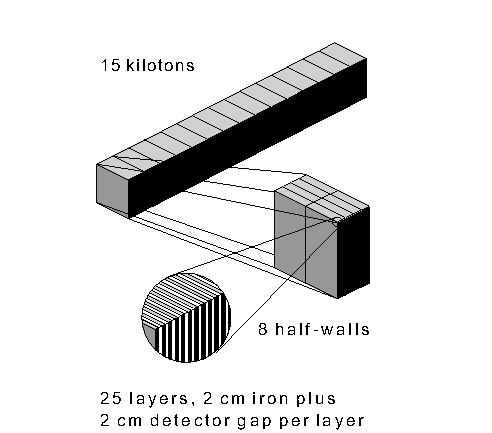
\includegraphics[width=0.75\linewidth]{node.pdf}
%         \caption{}
%     \end{subfigure}\hfill%
%     \begin{subfigure}[b]{0.5\textwidth}
%         \centering
%         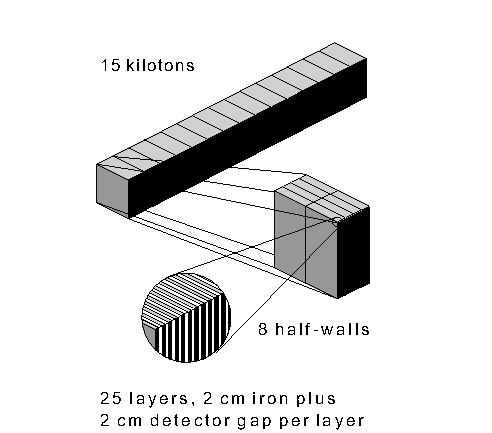
\includegraphics[width=0.75\linewidth]{node.pdf}
%         \caption{}
%     \end{subfigure}
%     \hspace*{\fill}%
%     \caption[]{This is an example figure caption}\label{fig:example_fig}
% \end{figure*}

% \begin{table}[htb]
%     \caption{This is the sample table caption.}\label{tableone}
%     \begin{tabular}[]{ccc} \hline
%         Index & Value 1 & Value 2 \\ \hline 1 & 0.1 & 0.6 \\
%         2     & 0.5     & 1.5     \\
%         3     & 1.2     & 3.5     \\ \hline
%     \end{tabular}
% \end{table}


% \printbibliography[title={REFERENCES}]

\end{document}
